\documentclass[tikz,border=6pt]{standalone}
\usepackage{amsmath,amssymb}
\usetikzlibrary{arrows.meta,decorations.pathmorphing,decorations.pathreplacing,calc}
\begin{document}
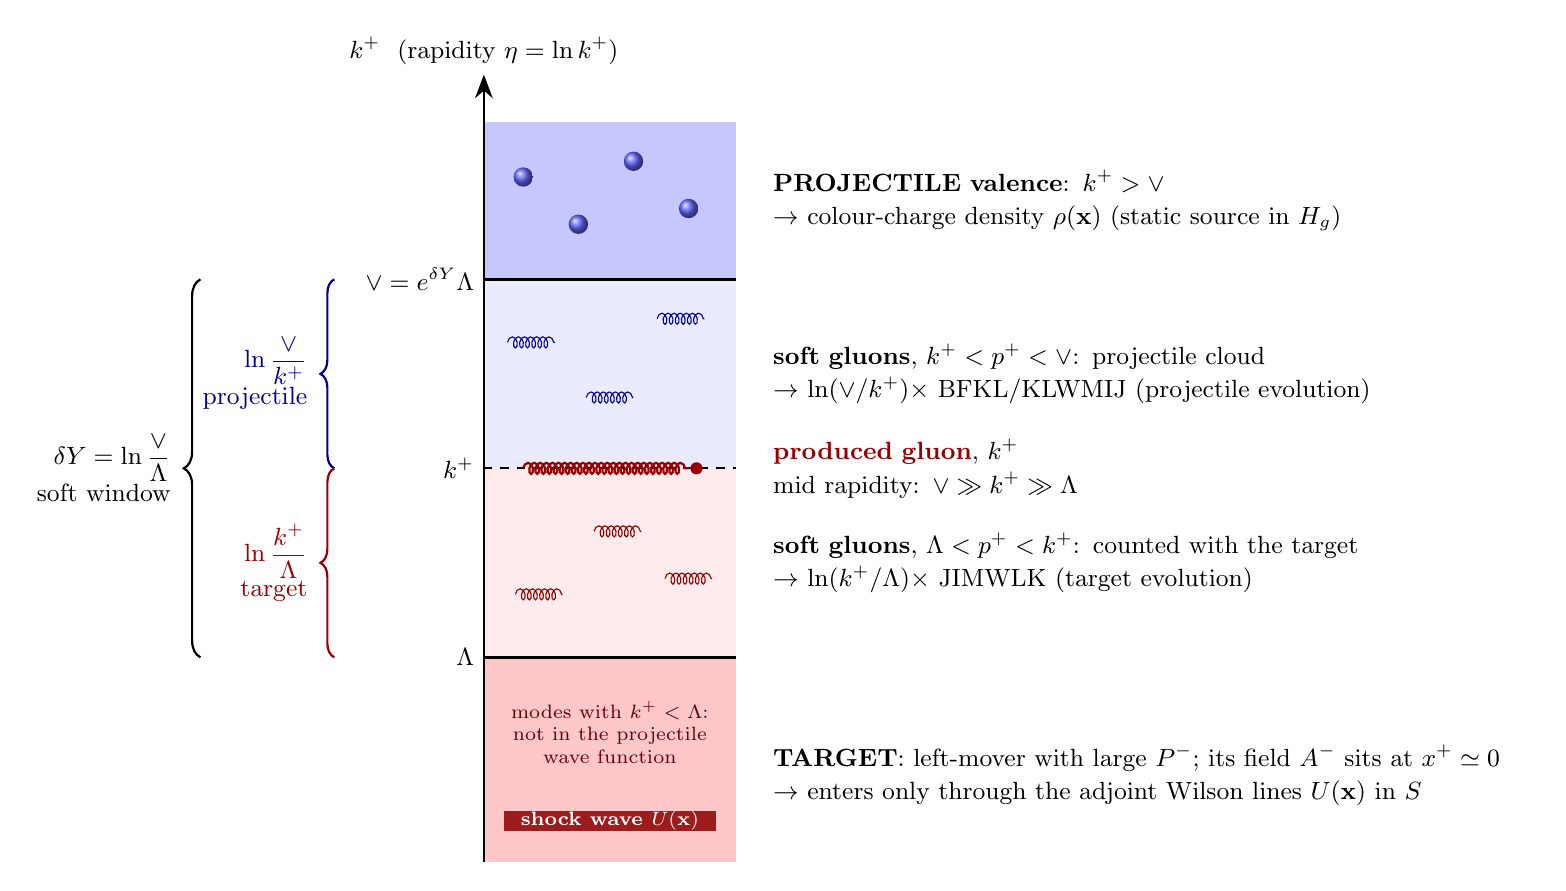
\begin{tikzpicture}[
    font=\small,
    lab/.style={anchor=west, align=left, text width=9.6cm},
    gluon/.style={decorate, decoration={coil, aspect=0.6, segment length=2.2pt, amplitude=2pt}},
  ]
  % ---- geometry
  \def\W{3.2}            % width of the bands
  \def\yV{6.0}           % vee
  \def\yK{3.6}           % produced gluon k+
  \def\yL{1.2}           % Lambda
  \def\yTop{8.0}
  \def\yBot{-1.4}

  % ---- bands
  \fill[blue!22]   (0,\yV) rectangle (\W,\yTop);
  \fill[blue!8]    (0,\yK) rectangle (\W,\yV);
  \fill[red!8]     (0,\yL) rectangle (\W,\yK);
  \fill[red!22]    (0,\yBot) rectangle (\W,\yL);

  % ---- axis
  \draw[-{Stealth[length=3mm]}, thick] (0,\yBot) -- (0,\yTop+0.6)
        node[above] {$k^+$\ \ (rapidity $\eta=\ln k^+$)};

  % ---- boundaries
  \draw[very thick] (0,\yV) -- (\W,\yV);
  \node[left] at (0,\yV) {$\vee=e^{\delta Y}\Lambda$};
  \draw[very thick] (0,\yL) -- (\W,\yL);
  \node[left] at (0,\yL) {$\Lambda$};
  \draw[dashed, thick] (0,\yK) -- (\W,\yK);
  \node[left] at (0,\yK) {$k^+$};

  % ---- produced gluon
  \draw[gluon, thick, red!60!black] (0.5,\yK) -- (\W-0.6,\yK);
  \fill[red!60!black] (\W-0.5,\yK) circle (2.2pt);

  % ---- valence: colour charges
  \foreach \x/\y in {0.5/7.3, 1.2/6.7, 1.9/7.5, 2.6/6.9} {
    \shade[ball color=blue!60] (\x,\y) circle (3.5pt);
  }
  % ---- soft projectile cloud
  \foreach \x/\y in {0.6/5.2, 1.6/4.5, 2.5/5.5} {
    \draw[gluon, blue!60!black] (\x-0.3,\y) -- (\x+0.3,\y);
  }
  % ---- soft gluons counted with the target
  \foreach \x/\y in {0.7/2.0, 1.7/2.8, 2.6/2.2} {
    \draw[gluon, red!55!black] (\x-0.3,\y) -- (\x+0.3,\y);
  }
  % ---- target shock wave
  \fill[red!55!black, opacity=0.85] (0.25,-1.0) rectangle (\W-0.25,-0.75);
  \node[white, font=\scriptsize\bfseries] at (\W/2,-0.875) {shock wave $U(\mathbf x)$};
  \node[red!40!black, align=center, font=\scriptsize] at (\W/2,0.25)
        {modes with $k^+<\Lambda$:\\ not in the projectile\\ wave function};

  % ---- labels (right)
  \def\xl{\W+0.35}
  \node[lab] at (\xl,7.0) {\textbf{PROJECTILE valence}: $k^+>\vee$\\[1pt]
        $\to$ colour-charge density $\rho(\mathbf x)$ (static source in $H_g$)};
  \node[lab] at (\xl,4.8) {\textbf{soft gluons}, $k^+<p^+<\vee$: projectile cloud\\[1pt]
        $\to$ $\ln(\vee/k^+)\times$ BFKL/KLWMIJ (projectile evolution)};
  \node[lab] at (\xl,\yK) {\textcolor{red!60!black}{\textbf{produced gluon}}, $k^+$\\[1pt]
        mid rapidity: $\vee\gg k^+\gg\Lambda$};
  \node[lab] at (\xl,2.4) {\textbf{soft gluons}, $\Lambda<p^+<k^+$: counted with the target\\[1pt]
        $\to$ $\ln(k^+/\Lambda)\times$ JIMWLK (target evolution)};
  \node[lab] at (\xl,-0.3) {\textbf{TARGET}: left-mover with large $P^-$; its field $A^-$ sits at $x^+\simeq0$\\[1pt]
        $\to$ enters only through the adjoint Wilson lines $U(\mathbf x)$ in $S$};

  % ---- rapidity-split braces (left)
  \draw[decorate, decoration={brace, amplitude=5pt, mirror}, thick, blue!60!black]
        (-1.9,\yV) -- (-1.9,\yK) node[midway, xshift=-6pt, left, align=right] {$\ln\dfrac{\vee}{k^+}$\\ projectile};
  \draw[decorate, decoration={brace, amplitude=5pt, mirror}, thick, red!60!black]
        (-1.9,\yK) -- (-1.9,\yL) node[midway, xshift=-6pt, left, align=right] {$\ln\dfrac{k^+}{\Lambda}$\\ target};
  \draw[decorate, decoration={brace, amplitude=6pt}, thick]
        (-3.6,\yL) -- (-3.6,\yV) node[midway, xshift=-7pt, left, align=right] {$\delta Y=\ln\dfrac{\vee}{\Lambda}$\\ soft window};
\end{tikzpicture}
\end{document}
